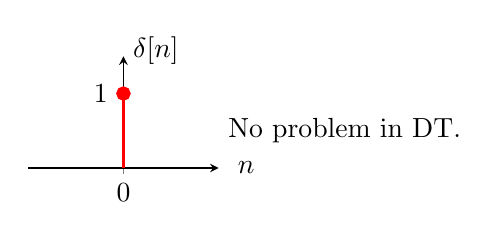
\begin{tikzpicture}
	\begin{axis}
	[
		name=axis1,
	       width=4cm,
	       height=3cm,	
		axis y line=middle,
		axis x line=bottom,
		ymin=0,ymax=1.5,
		xmin=-4,xmax=4,	
		xlabel=$n$,
		ylabel={$\delta[n]$},	
		xtick={0},
		xticklabels={0},
		ytick={1},
		yticklabels={1},
		every axis x label/.style={at={(ticklabel* cs:1.05)},    anchor=west},
		every axis y label/.style={at={(ticklabel* cs:1.05)},    anchor=west},	
		clip=false,
	]
	\addplot[ycomb,  red, very thick, mark=*,] coordinates {(0,1)};
	\node at (axis cs:4, 0.5) [anchor=west] {No problem in DT.};
	
	\end{axis}
\end{tikzpicture}